\section{Arquitetura do sistema}
\begin{figure}[H]\centering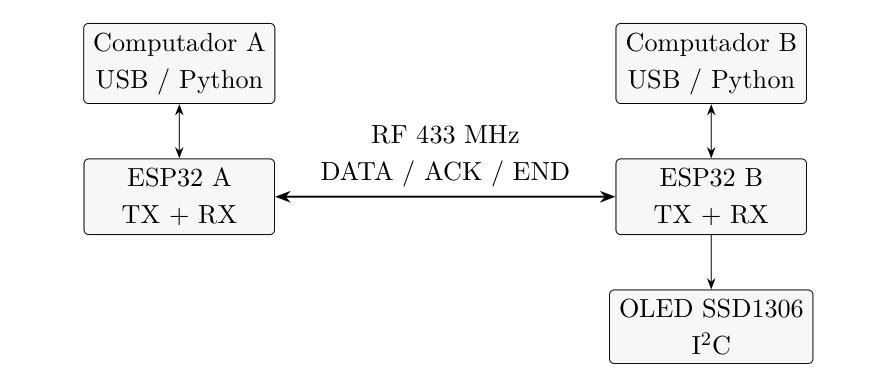
\includegraphics[width=\linewidth,height=210pt,keepaspectratio]{figuras/arquitetura.png}\caption{Arquitetura funcional do enlace bidirecional. Fonte: relatório técnico anterior.}\label{fig:arquitetura}\end{figure}
O computador A envia comandos e bytes por USB ao ESP32 A. O microcontrolador organiza os dados, calcula o FCS, codifica e aciona o transmissor RF. O receptor RF do circuito B entrega os sinais ao ESP32 B, que decodifica, verifica a integridade e confirma os quadros válidos pelo rádio. O computador B recebe o conteúdo reconstruído por USB; o OLED apresenta a informação localmente.

Na direção B \ensuremath{\to} A, os mesmos papéis são invertidos. Cada circuito possui alimentação e referência de terra locais. Não existe conexão física de dados entre A e B. O enlace é utilizado em semiduplex: a aplicação inicia uma sessão de envio por vez para reduzir colisões.

\begin{table}[H]\centering\small\caption{Camada / Função}\label{tab:1}
\rowcolors{2}{tcdlight}{white}\begin{tabularx}{\linewidth}{>{\hsize=0.5567\hsize\linewidth=\hsize\raggedright\arraybackslash}X>{\hsize=1.4433\hsize\linewidth=\hsize\raggedright\arraybackslash}X}
\rowcolor{tcdtablehead} \textcolor{black}{\textbf{Camada}} & \textcolor{black}{\textbf{Função}} \\
Computador /\allowbreak  Python & Interface com usuário, conversão de imagem, USB, reconstrução e hashes. \\
ESP32 /\allowbreak  firmware V7 & Enquadramento, CRC-8, codificação 4B6B, ARQ e controle de sequência. \\
RF TX/\allowbreak RX & Transporte de sinais por rádio de 433 MHz. \\
OLED I\textsuperscript{2}C (somente B) & Apresentação local de texto e imagem monocromática. \\
\bottomrule\end{tabularx}\end{table}
